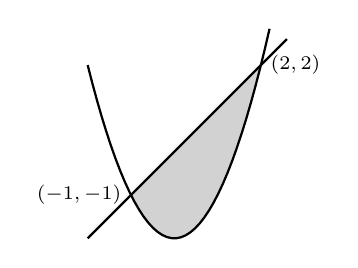
\begin{tikzpicture}[scale=0.55]
\fill[gray!35] plot[domain=-1:2,samples=40] (\x,{\x*\x-2}) -- (2,2) -- (-1,-1) -- cycle;
\ax{-2.4}{2.8}{-2.5}{3}
\draw[thick,domain=-2:2.2,samples=40] plot (\x,{\x*\x-2});
\draw[thick] (-2,-2)--(2.6,2.6);
\node[right] at (2,2){\scriptsize $(2,2)$}; \node[left] at (-1,-1){\scriptsize $(-1,-1)$};
\end{tikzpicture}